\documentclass{article}
\usepackage[utf8]{inputenc}

\title{Autoencoders}
\author{Mihir Patel}
\date{March 2018}

\usepackage{natbib}
\usepackage{graphicx}
\usepackage{amsmath}

\begin{document}

\maketitle

\section{Introduction}
One of the issues with machine learning when going from raw data is too many input variables. The sheer number of inputs makes it hard to train and often can lead to overfitting (see curse of dimensionality). Autoencoders were originally proposed as a method of reducing dimensions and extracting higher level features that we know for sure contain most if not all of the information. It can be thought of as storing the information in a more efficient and meaningful way.

\section{The Structure}
\begin{center}
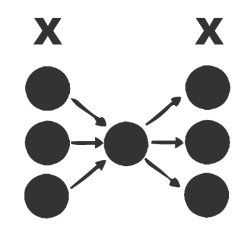
\includegraphics[scale=0.50]{autoencoders}
\end{center}
\subsection{Definition}
Autoencoders, instead of narrowing down like most networks, instead are shaped like an hourglass. When trained, the output should be exactly the same as the input. So if we feed the network a picture of a cat, it will give the exact same picture back. This forces the network to try to maintain all of the information through each layer and not lose anything. However, in the middle it gets narrower! This means it must find a more effective way of storing the same amount of information. The first half that converts the information into the narrow region is called the encoding portion and the second half that converts it back into the original information is called the decoding portion.

\section{Example: Number Systems}
This can be a bit tricky to wrap our head around, so lets start with an example. Say we have a network that takes in 8 inputs. Each input node represents a number. So if we want to pass the number 1, we make the first neuron a 1 and the rest 0s. If we want to pass the number 2, we make the second neuron a 1 and the rest 0s. And so on. This process is actually called one-hot encoding. We then create a network with a very simple structure. Besides the input layer with 8 nuerons, we will add a hidden layer with 3 neurons and another output layer with 8 neurons. Now we train the network to spit back out the same exact input. This means it MUST learn to take the input and store it in only 3 neurons if it wants to learn. In this case, it can just learn binary! One of the three hidden ones represents +1, another represents +2, and another represents +4. This way, we can represent 8 different numbers ($2^3$).

\section{Applications}
Standard autoencoders are useful for pretraining low levels of a deep network. In the past, without high-end GPUs, autoencoders would be used to extract out basic features from information. The input would be passed to train a shallow autoencoder. Then, the decoding portion would be chopped off and the network would be made deeper, with even smaller layers being added in the middle along with a new decoder. This would be repeated as long as needed to train these low levels.

\section{Adding Convolutions}
One of the biggest uses of autoencoders early on was images. Images have lots and lots of raw information (pixels) and easily identifiable features that can better represent the image. So naturally, the next step was in adding convolutional layers to autoencoders. However, to do this, we also need deconvolutional layers and unpooling. This process is called upsampling.

\section{Unpooling}
\begin{center}
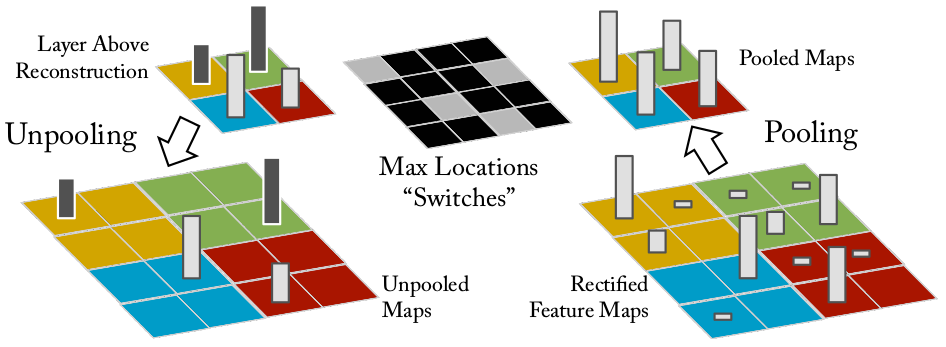
\includegraphics[scale=1.0]{unpooling}
\end{center}
\subsection{Definition}
The first step in this process is reversing pooling. Unfortunately, this is basically impossible as we've thrown away the information from the other squares in the pooling process. Essentially, if we are unpooling a 1x1 region to a 2x2 region (reversing 2x2 pooling), we first move the 1x1 region to the right location in the 2x2 box. This is done by using switches, which essentially store the original location from the pooling. Basically, each pooled region takes not only the value, but the original location it was in before the pool, which is then used in the unpooling. The remaining squares are filled with 0s.

\section{Deconvolutions}
\begin{center}
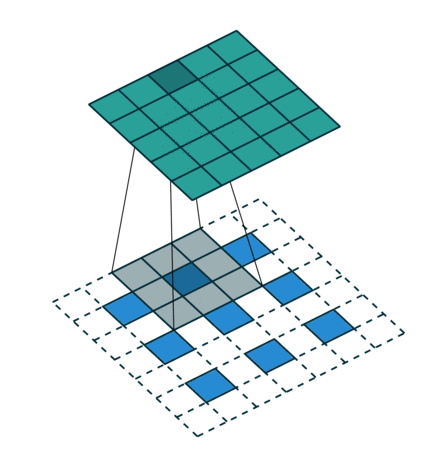
\includegraphics[scale=.50]{deconv}
\end{center}
\subsection{Definition}
The next step is deconvolutions. Normally, the bottom would be the input and the top is the generated values from the kernel. In this case, you have the green region and want the bottom. To do this, you take the kernel and multiply every single location with the pixel value you are deconvolving. Where there are overlaps, you sum the values. Typically, high stride lengths are used to minimize overlap. In this image, each blue pixel is where the deconvolutional kernel is applied to. Let's look at an example. Our kernel is...

\[
\begin{bmatrix}
    3 & 4 \\
    1 & 1
\end{bmatrix}
\]

We can apply it to the 2x2 following image matrix with a stride length of 2.

\[
\begin{bmatrix}
    1 & 2 \\
    5 & 9
\end{bmatrix}
\]
\[
->
\begin{bmatrix}
    3 & 4 & 0 & 0 \\
    1 & 1 & 0 & 0 \\
    0 & 0 & 0 & 0 \\
    0 & 0 & 0 & 0
\end{bmatrix}
+
\begin{bmatrix}
    0 & 0 & 6 & 8 \\
    0 & 0 & 2 & 2 \\
    0 & 0 & 0 & 0 \\
    0 & 0 & 0 & 0
\end{bmatrix}
+
\begin{bmatrix}
    0 & 0 & 0 & 0 \\
    0 & 0 & 0 & 0 \\
    15 & 20 & 0 & 0 \\
    5 & 5 & 0 & 0
\end{bmatrix}
+
\begin{bmatrix}
    0 & 0 & 0 & 0 \\
    0 & 0 & 0 & 0 \\
    0 & 0 & 27 & 36 \\
    0 & 0 & 9 & 9
\end{bmatrix} 
\]
\[
= 
\begin{bmatrix}
    3 & 4 & 6 & 8 \\
    1 & 1 & 2 & 2 \\
    15 & 20 & 27 & 36 \\
    5 & 5 & 9 & 9
\end{bmatrix}
\]

And presto, we have just deconvolved the image using our filter!

\section{Masking}
\begin{center}
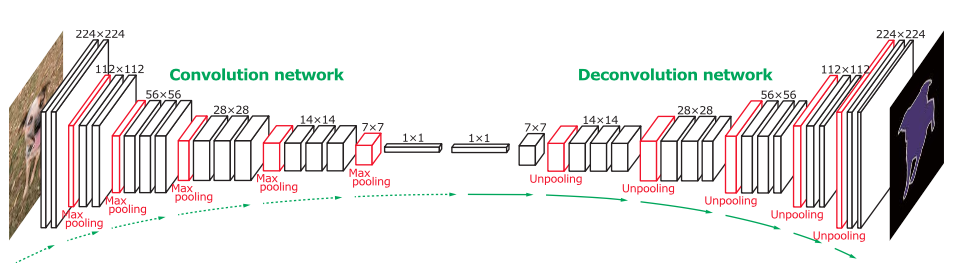
\includegraphics[scale=0.30]{masking}
\end{center}
\subsection{Definition}
Eventually, people realized deconvolutional layers can be used for much more. By being able to regenerate the image, you can do much more complex things such as identifying objects at a pixel level that otherwise would be very difficult to do. A common approach is to reverse a convolutional network, in this case VGG, and build a decoding portion to regenerate the mask. A similar approach is used in mask-RCNNs for multi-object segmentation. All kinds of similar image manipulations (such as denoising) can be done using deep learning through this method.

\section{Sequence to Sequence Autoencoders}
Another type of autoencoders which is highly used by Google Translate is sequence to sequence autoencoders. We won't go too much into depth into this because it quickly becomes very complicated, but essentially the idea is that autoencoders can convert sequences. One common usage is language translation, where the input would be say something in English and the output would be something in Chinese. That internal middle  part can essentially learn a "universal" language. This universal language contains all of the semantic information of language and can be translated to and from both English and Chinese. This turns out to be very difficult to do and several approximations are made, but autoencoders have been shown to perform leagues beyond past methods.

\end{document}
